\documentclass[authoryear,preprint]{elsarticle}

\usepackage[utf8]{inputenc}
\usepackage{amsmath}

\title{A Refined Wave Resource Assessment Methodology: Application to U.S. Waters}
\author{Levi Kilcher, Gabriel-Garcia Medina, Zhaoqing Yang, Aidan Bharath}
\date{October 2019}

\showboxdepth=5
\showboxbreadth=5

\newcommand{\degrees}[0]{\ensuremath{^\circ}}

\begin{document}

\begin{abstract}
TBD...
\end{abstract}

\maketitle


\section{Introduction}

Over the last decade global interest in wave energy has grown considerably, with the Ocean Energy Systems executive committee setting a goal of 300GW of installed ocean energy capacity by 2050 \citep[]{huckerbyInternationalVisionOcean2017}. This has been driven by concerns about greenhouse-gas driven climate change, carbon-based energy price volatility, and a growing understanding of the value of diversifying energy sources. Wave energy technology is still at an early-stage of technology development, with a wide-range of device archetypes under active development \citep[]{babaritOceanWaveEnergy2017}. 

During these early years of wave energy research and development, it has been important to quantify the wave energy resource so that decision makers can understand the market opportunity of this new technology. Wave energy resource assessments can be divided into two types:

\begin{enumerate}
\item Global, regional, and national assessments (hereafter, collectively ‘regional’ assessments) that quantify the total theoretical resource for a relatively long section of coastline (i.e., $>$O(100 km)). Most importantly, regional assessments provide an estimate of the total power available in the wave field for the region of interest.
\item Site resource assessments provide a collection of resource details that are useful for estimating the site’s power production potential and for project design. Most importantly, site assessments provide a joint probability distribution of wave energy period and\ wave height that can be used with a device ‘power matrix’ to calculate the project’s annual energy production.
\end{enumerate}

These assessments are valuable for different purposes. Regional assessments are the foundation of more detailed market research (such as site assessments), they motivate regional planning, and provide justification for government investment \citep[e.g., ][]{EPRIwaveresource2011,gunnQuantifyingGlobalWave2012,regueroGlobalWavePower2015,motaWaveEnergyPotential2014}. Site assessments provide data needed for feasibility and design studies that are critical to obtaining project financing and investment \citep[]{robertsonCharacterizingShoreWave2014,iglesiasWaveEnergyPotential2009}.

The methodologies of these assessment types are currently distinct because the marine energy community has not yet developed a unified assessment method that provides the data for both (large-scale total energy-flux and also the power matrix at a site). 
A detail that confounds unifying these two approaches is the fact that wave energy flux is a directional quantity. This means that - in order to avoid double counting - regional totals must account for the directionality by performing a line-integral. On the other hand, for site assessments involving sparsely positioned omni-directional devices (i.e., devices that absorb energy equally in all directions), wave directionality does not have a significant impact on the project’s technical potential. With this understanding and motivated by a desire to address the needs of the industry where it is now (i.e., most projects involve 10 or less devices), the first edition of the International Electrotechnical Commission’s resource assessment technical specification does not explicitly account for directionality or array effects \citep[]{internationalelectrotechnicalcommissionPart101Wave2015}. While the IEC site assessment methodology has these limitations, it has been developed through a consensus process that encourages widespread adoption and consistency. The methodology for regional assessments, on the other hand, has not been developed by consensus, which has led to inconsistent approaches and confusion when comparing results.

We undertake the task of establishing a consistent regional wave resource assessment methodology by first pointing out that the wave resource for a region of water is composed of two parts (Figure \ref{fig:map01}): 1) the ‘remote resource’, which is the wave energy created by winds outside the region — e.g., by storms in the distant open-ocean — that propagates into the region \citep{gunnQuantifyingGlobalWave2012, hemerRevisedAssessmentAustralia2017}, and 2) the ‘local resource’, which is the wave energy created by winds within the region itself. The majority of existing wave resource assessments have considered the remote resource only. While neglecting the local resource may be valid in specific scenarios, the fact that it has been ignored (often implicitly) has raised many questions and led to confusion about wave resource assessment methodology. The primary objective of this work is to quantify both the remote and local resource explicitly, and thereby resolve lingering questions regarding the details of regional resource assessment.

\begin{figure}[ht]
  \centering
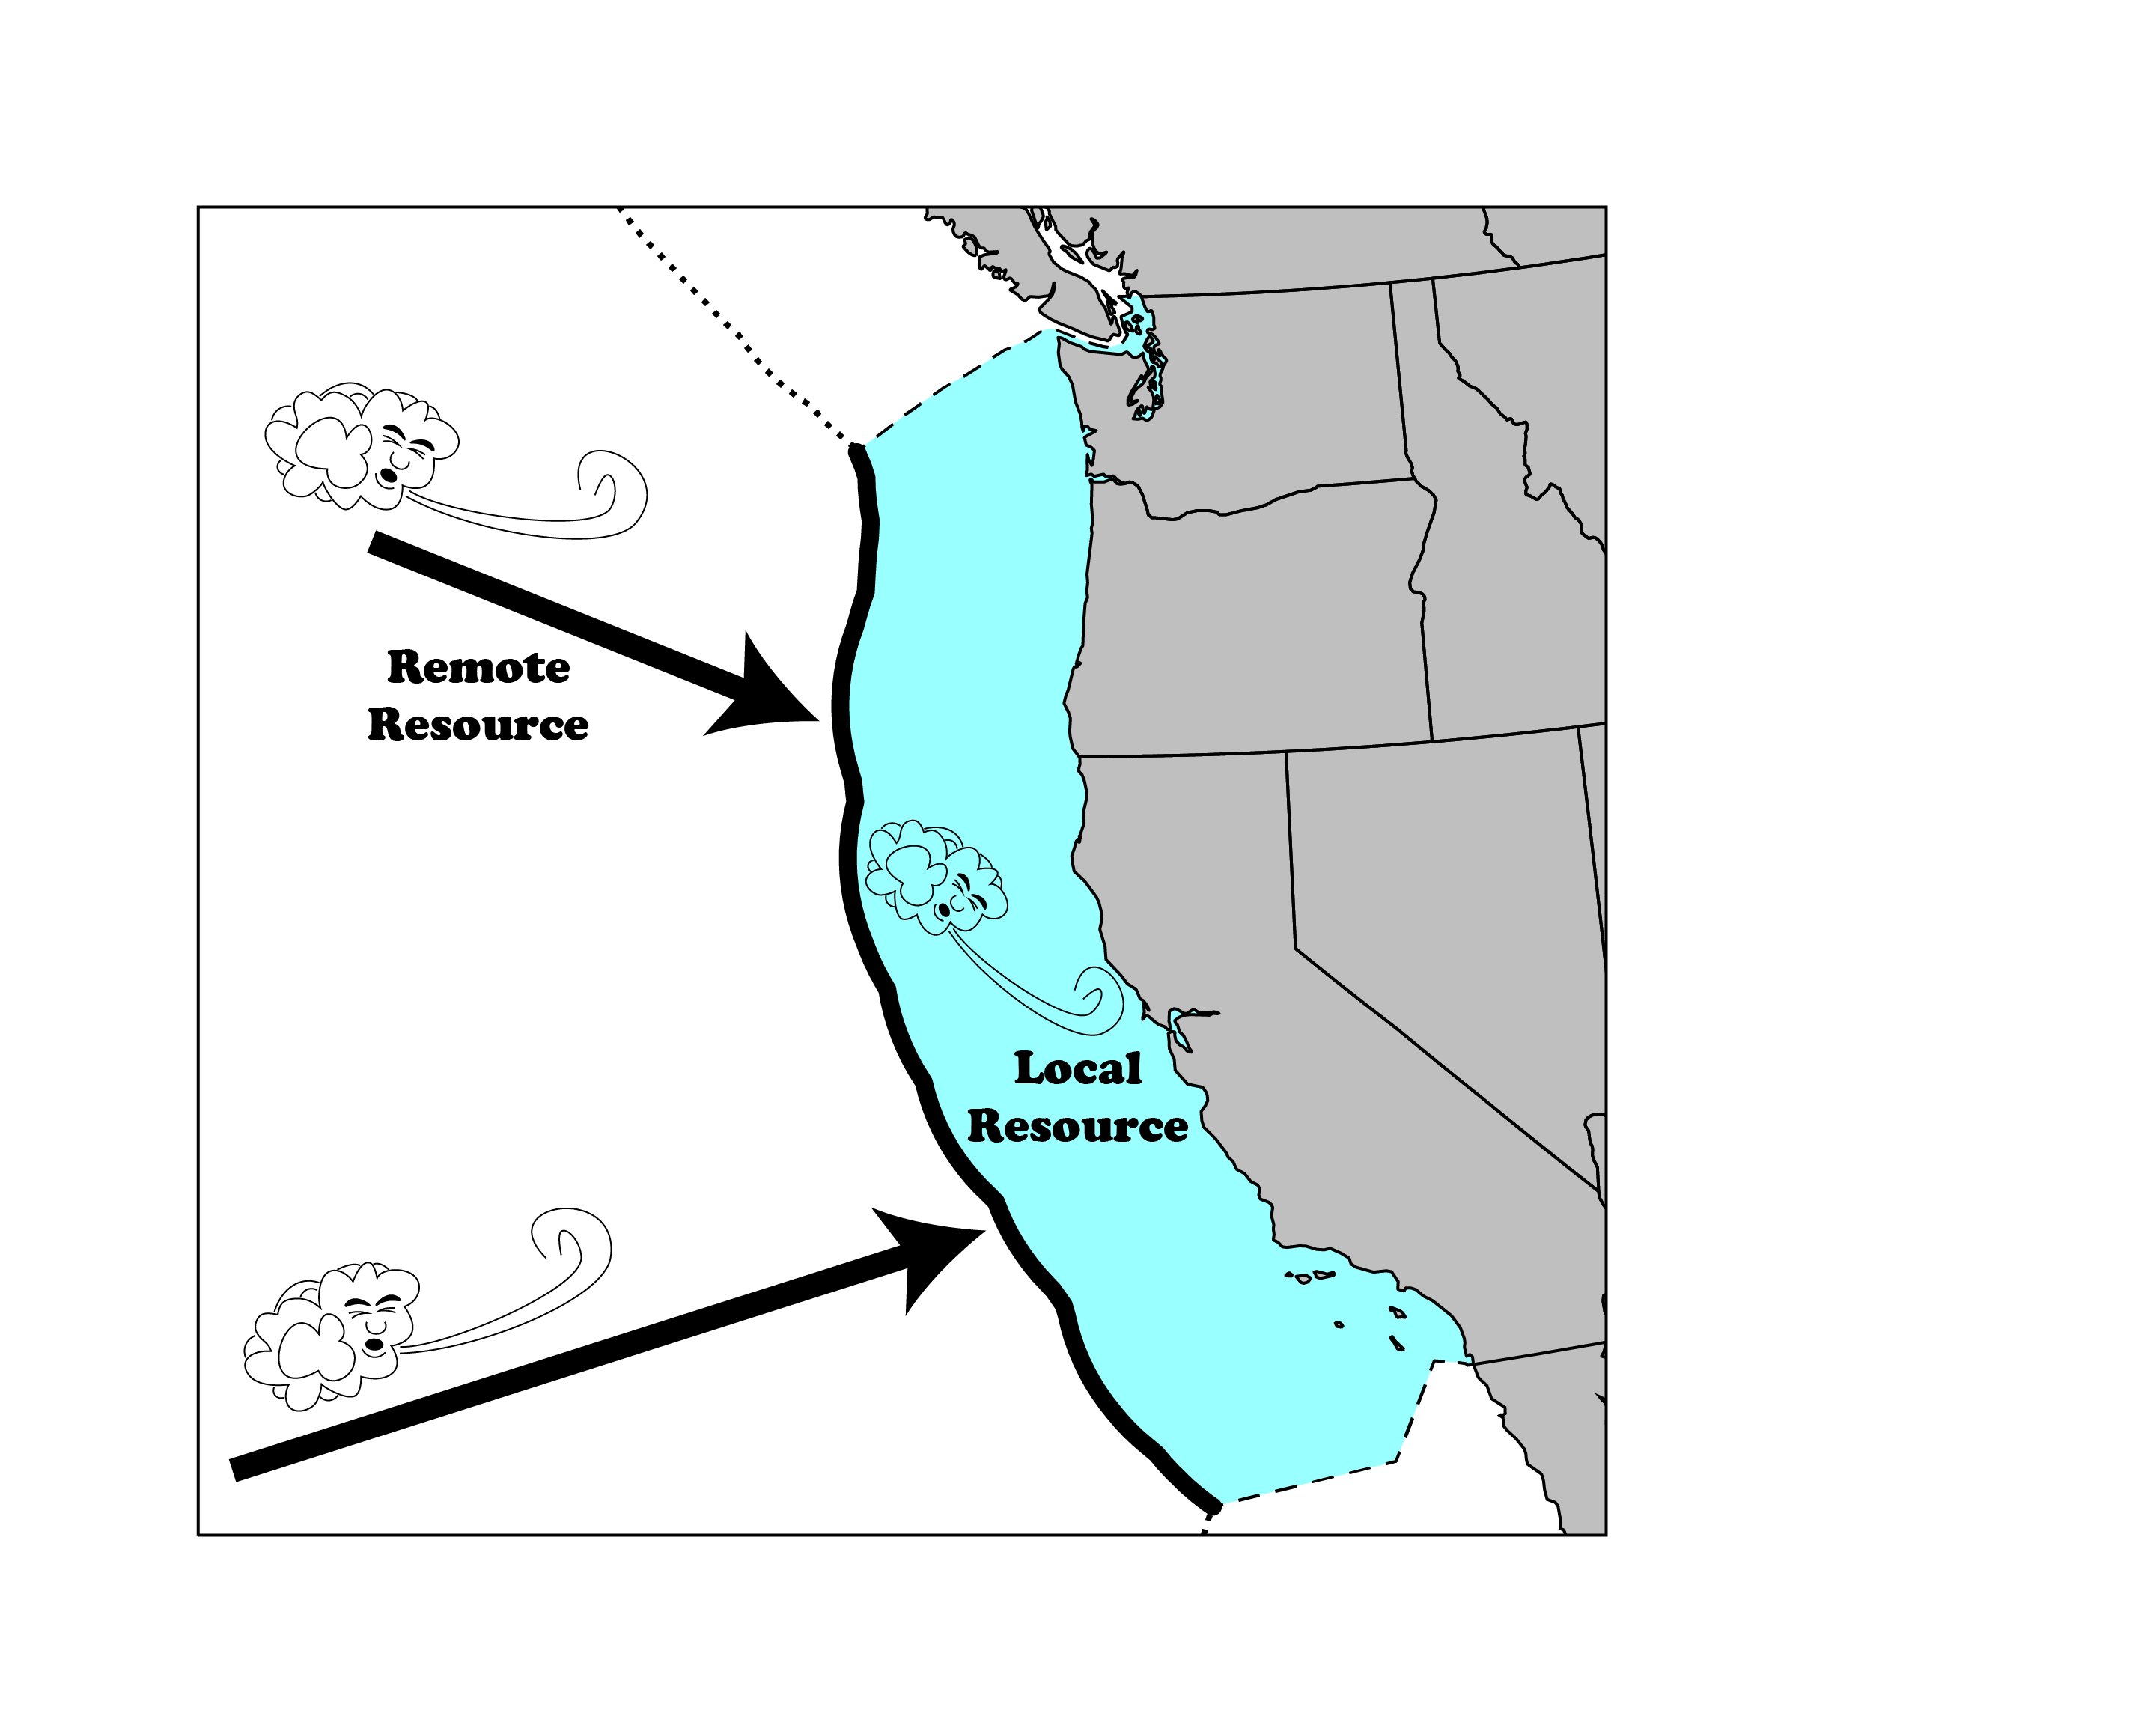
\includegraphics[width=0.9\linewidth]{../diagram/EEZ_contour03_edit01.png}
  \caption{A diagram depicting the U.S. West Coast’s ‘remote’ (arrows) and ‘local’ (cyan) resource.}
  \label{fig:map01}
\end{figure}

A secondary objective of this work is to provide a refined estimate of the U.S. wave resource based on this new method, and new model results. A tertiary objective is to provide guidance that helps address limitations in site assessment, which we hope will eventually lead to a unified methodology for site and regional wave resource assessment.

These objectives are accomplished by first discussing the details of regional assessments (section 2), and then presenting our proposed approach (section 3). In section 4, we present the results of this approach applied to each region of the U.S. coastline in comparison to alternate methods that have been used. Section 5 provides a detailed discussion of the results, including a justification for the proposed approach, and a summary of how the proposed approach can be applied in different scenarios. We conclude with a summary of results, the proposed methodology, and a view toward how to unify wave energy site and resource assessment.

\section{Background}

Ocean surface waves are generated by wind blowing across the ocean surface. The energy is transferred from the atmosphere to the ocean by the friction of wind on the ocean surface, and by pressure differentials associated with the wind blowing across the wave crests \citep[]{phillipsDynamicsUpperOcean1980,youngWindGeneratedOcean1999}. At the site of wave generation - in a storm, for example - waves of many frequencies, $f$, are generated. As these waves propagate across the ocean surface they cross-paths with waves from other locations. Thus, at any point on the ocean surface, the sea-state is composed of a mix of waves of differing frequencies and coming from different directions. The distribution of wave energy as a function of frequency (or period), and direction is quantified by the ‘directional spectrum’ (Figure \ref{fig:dirspec}).

Regional wave resource assessments are typically accomplished using spectral wave energy simulations. These models simulate wave energy propagation according to wave energy kinematics (i.e., at the group velocity), and they contain ‘source and sink’ terms to estimate the generation, evolution (i.e., non-linear interactions that transfer energy between frequencies), and dissipation of spectral wave energy in space and time (Booij et al. 1999; The WAVEWATCH III Development Group (...). These terms are based on empirical measurements, and are typically functions of the wind forcing and bathymetry (both of which must be supplieas input to the model).

There is broad consensus that these models should: utilize modern physics packages (source and sink terms), span several decades to account for inter-annual variability, and be validated against several measurement points in the region of interest. While there is consensus and agreement on these points, there has been considerable confusion regarding how to use the model data to compute resource totals. This confusion has three primary sources:


\begin{figure}[ht]
  \centering
  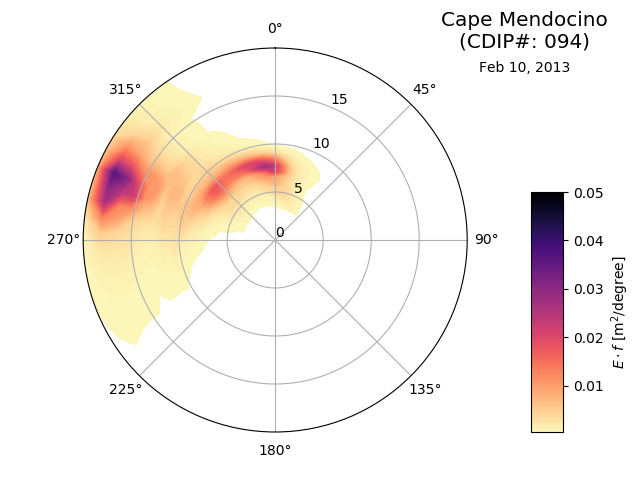
\includegraphics[width=0.9\linewidth]{../fig/dirspec.png}
  \caption{Directional spectrum}
  \label{fig:dirspec}
\end{figure}

\begin{enumerate}
\item Waves can come from multiple directions at the same time, and many WEC types can absorb energy equally from all directions. How does one reconcile this detail of individual devices with the need to account for wave-flux directionality when computing a line-integral in a regional assessment?
\item Local winds can generate energy inshore of the selected contour. How does one account for that energy? This issue is confounded by the fact that source-terms are proportional to the wave spectrum (wave size).
\item Wave models are typically configured to propagate wave energy throughout the domain (not absorb at the chosen boundary). How does one know whether or not wave energy crossing the boundary has already been ‘counted’ at a different location and time?
\end{enumerate}

Each of the above issues are considered in more detail in the following subsections.

\subsection{Wave directionality}

\begin{figure}[ht]
  \centering
  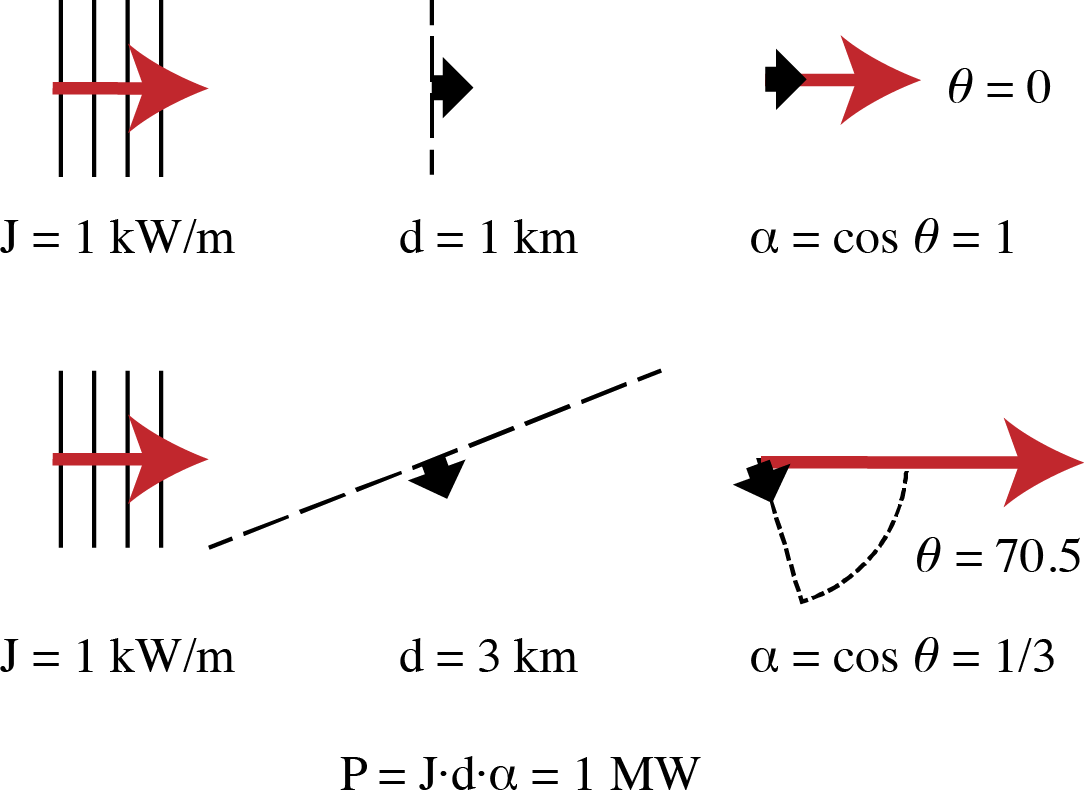
\includegraphics[width=0.7\linewidth]{../diagram/Dot-Product_Schematic01}
  \caption{A schematic depicting the importance of directionality in computing energy-flux totals. The upper and lower sequence of pictures depict the same wave (left) encountering a contour at different angles (middle). The red-arrow depicts the wave direction, and the black arrow the contour-normal. The angle between these vectors is $\theta$ (right).}
  \label{fig:directionality}
\end{figure}

Because wave energy flux is a vector (directional) quantity, it’s sum must be computed using a method that properly accounts for the directionality. Figure 3 illustrates this point: in both the top and bottom rows, the total wave energy flux in the 1 km wide wave is 1 MW. If, however, the wave-direction is unknown and one were to naively multiply the wave-flux magnitude by the length of the contour (i.e., incorrectly assume that the wave flux is perpendicular to the contour), the lower example will overestimate the resource by a factor of 3. Thus it is important to utilize a ‘dot-product’ when computing wave-flux totals. When waves from different directions are arriving at a location simultaneously, the dot-product should be computed for each wave crossing the contour, and then these totals summed separately.

However, in order to reduce the data-storage burden, wave models are often configured to store summarized (incomplete) information. This may mean that no directional information is preserved in the model output (e.g., only wave height and period is available), or perhaps only the ‘average wave direction’ or the ‘direction of the largest wave’ are available. Resource assessments based on these kinds of data will contain errors due to incorrectly accounting for wave direction. The magnitude and sign of this error depends on the details of the data limitations, and the assumptions that are made to accommodate these limitations.

An earlier U.S. wave resource assessment suggested that directionality could be ignored because many WECs (e.g., a ‘point absorber’) can absorb energy equally from any direction (Jacobson, Hagerman, and Scott 2011). While this reasoning is true for a single device, it breaks down when considering an array of devices that are close enough together to capture all of the incident resource. It is, after all, the purpose of resource assessment to estimate the total available resource.

In particular, when the devices are packed close enough together to capture all incoming wave energy, some devices - for certain wave directions - will be wholly or partially in the ’shadow’ of others. The shadowed (i.e., ‘down wave’) devices will not be subjected to the full resource intensity because the shadowing (‘up wave’) devices will have captured some fraction of the incident resource (Babarit 2013). The details of which devices are shadowed vs. shadowing depends on the details of the array layout and the incident wave direction. But this is entirely the point: wave directionality is as important for tightly-spaced arrays of point absorbers as it is for directional device types. For the purposes of - and at the scale of - regional resource assessment, we can ignore the details of device type and array configuration and instead treat the “array” as a line that absorbs all incoming wave energy (i.e., using a dot-product).

We use a one-way dot-product to compute wave energy flux 'into' the box \citep[]{gunnQuantifyingGlobalWave2012}. 
% What is the right amount to discuss the 'directional method' issue? Reference the EPRI 2011 RA, and the NAS Review? Then, ...

\subsection{Local Resource}

To our knowledge, all prior wave resource assessments have been completed by considering the remote resource only. That is, by estimating wave-energy flux across a boundary that is selected to be representative of the coastline of interest. This approach has raised the question: what about waves that are generated inshore of the chosen boundary (hereafter, the ‘locally generated energy’)? The answer has usually been that this contribution is believed to be small, but few have undertaken the task of quantifying it.

The rationale for neglecting the locally generated energy seems to have been based on some combination of: a) it can’t be calculated from the data I have, b) the ocean surface inshore of the contour I’ve selected is very small compared to the rest of the ocean (so the local energy should be small compared to the remote energy), and c) the local generation is likely to be dominated by relatively short-period waves, which are lower energy (per wave height). While this reasoning is reasonable for the first generation of wave resource assessments, we think it is time to consider this term explicitly in wave resource assessments.

We configure our WW3 model to write-out the wind-input and dissipation source terms for the entire domain of interest. These terms have units of power unit-crest-length, per unit fetch-length (e.g., W/m2). Thus, an area integral of these terms - over the region of interest - provides an estimate of the rate of energy input from the wind to the water. Adding these terms to the wave resource budget has three details worth noting, described in the following subsections.

\subsubsection{Source-term directionality}

First, we point out that - while the source terms are directional - this directionality is unimportant for the purposes of resource assessment. This may be surprising to the reader, considering the importance we have attributed to the directionality of the ‘remote’ resource, but we point out that this is an entirely different term involving an area-integral rather than a line integral. In the case of the line-integral, wave directionality was important relative to the boundary line (edge of the array of devices). Now, inside the boundary, we presume for the purposes of resource assessment that devices essentially ‘blanket’ the ocean so that wave energy can be extracted as soon as it is created. Within the boundary, as wave energy is added to the wave field, the directionality of that energy is unimportant to calculating the total there are devices in all directions.

To put the above in the terms of control volume mathematics (two-dimensional): the rate of change of a quantity (e.g., energy) inside a boundary is equal to the line-integral of the flux across the boundary, plus the area-integral of the sources (and sinks) of that quantity across the entire volume. This is exactly what we’re doing here, we’re adding a line-integral of fluxes and an area integral of source-terms to get a total.

\subsubsection{Source-term non-linearity}

Second, the magnitude of the input source term is proportional to the amplitude of the wave energy spectrum. That is, larger waves grow faster than small ones (i.e., wave growth is non-linear). This is a fundamental concept of wave growth, but it complicates the task of calculating the ‘locally generated energy’. The simplest scenario would be to run a “lake” simulation, in which the simulation is configured so that no remote wave-flux crosses into the study-area (i.e., it is all absorbed at the boundary). Then one simply lets the local waves build within the study-area based solely on local generation, and calculate that total power.

In this simplistic approach, we are imagining a scenario in which all ‘remote’ wave energy is absorbed at the offshore boundary of the study-area. However, one wonders if it would be better to allow the waves to propagate into the study-area so as to increase the magnitude of the source terms (which will be larger for these larger waves). Furthermore, because the source terms are proportional to the wave-spectrum, the frequency dependence of the source terms is also highly dependent on the wave-field. This makes calculating the source-term resource particularly challenging if one plans to weight frequency bands differently (e.g., ignore very-high and very-low frequency bands). In this work we do not weight frequency bands differently.

For the purposes of RA, this essentially becomes an optimization problem of ‘where and when’ to extract energy to maximize total extractable power (i.e., maximize source-term wave growth relative to dissipation terms). From a purely energetics standpoint (neglecting the frequency content of the waves, and the frequency dependence of wave converters), wave energy would ideally be extracted just ‘down-wave’ from a location where winds have added energy to the wave-field (i.e., before dissipation begins to reduce the total wave energy). However, because storms move around the practicality of harvesting wave energy just downstream of generation sites (storms) is probably unrealistic.

From a practical standpoint, these details are relatively unimportant until we actually possess the technology to extract wave energy on large scales. Rather than optimizing power extraction siting, we can estimate the range of source terms by assuming that the ‘lake’ simulation provides a lower-bound estimate of the source terms, and that a simulation with the full remote waves present inside the study-area provides an upper-bound estimate of the source terms.

\subsubsection{Source-term accuracy}

Finally, there is considerable debate on the topic of the accuracy of the formulation of the source terms, and new source term formulations are frequently being proposed. In this work, we use the ST4 package because... And, we assess the uncertainty in source terms by looking at the differing magntiudes of the terms with/without remote wave energy. Some authors have shown that while the magnitude of the sum of the input and dissipation terms seems reasonable, the values of these terms individually may have larger error (Moghimi et al. 2016). This means that, until we have more confidence in the values of these terms, results based on them should be carefully considered...

To summarize, we believe that considering the source terms is an important step toward a more comprehensive wave resource assessment. And, while there are still outstanding issues to be investigated (namely: the importance of source-term non-linearity and accuracy), estimating the uncertainty in these terms is useful for a more complete picture of the wave resource uncertainty as a whole.

\subsection{Has this wave been counted?}

\begin{figure}[ht]
  \centering
  \includegraphics[width=\linewidth]{../diagram/schematic03.png}
  \caption{A schematic of wave energy flux crossing a contour for the scenarios depicted by arrows A, B, C, D, E. The diagram depicts three distinct methods for summation: ‘traditional’ (pink), ‘bi-directional’ (orange), and ‘one-way’ (cyan). At each arrow intersection, the ‘+’ or ‘-’ indicates whether that method adds to or subtracts from the total depending on the direction relative to the contour (upper left legend). At the end of each arrow, the total sum for each method is indicated (ideally each wave should be counted ‘1’ time). The table at lower-right summarizes these totals.}
  \label{fig:wave-counting}
\end{figure}

The third source of confusion in calculating wave resource totals is perhaps best summarized by the question: “Has this wave been counted already?” This issue is related to the details of the use of the dot-product (a.k.a., ‘scalar product’) for calculating wave resource totals. The ‘traditional’ dot-product of two vectors a and b is:

\begin{align}
  \vec{a} \cdot \vec{b} = a b \cos(\theta)
\end{align}

Where $a$ and $b$ are the magnitudes of the vectors $\vec{a}$ and $\vec{b}$, respectively, and $\theta$ is the angle between them. This equation properly accounts for the wave energy that propagates across the contour and is eventually dissipated on the coastline (Figure \ref{fig:wave-counting}, arrow A). It also works for waves that cross a boundary an odd number of times on their way toward the coastline (e.g., arrows B and D). However, waves that cross the boundary an even number of times are not counted at all (arrow C, traditional total of 0), and waves that cross the boundary in the ‘outward’ direction are subtracted from the total (arrow E, traditional total of -1), both of which are not the desired result.

This problem arises from the fact that there is no way to know whether wave energy crossing at one location has already been counted at a different location. The traditional dot-product calculates a ‘net’ flux into the box, but it does not include the wave energy that passes through the region or originates within it (both of which could be captured by devices inside the region).

For example, if wave energy propagates past an island, it might pass into and then out of the study-area. At the point where it passes in, the energy in the wave will be added to the total, but it will be subtracted again where it passes back out of the resource area. Thus, using the traditional dot-product method, this wave-group will not be counted in the resource total. To address this issue, many wave resource assessments have used a ‘one-way’ dot product:

\begin{align} \label{eqn:oneway}
\begin{split}
  \vec{a} \cdot \vec{b} & = ab \cos(\theta) \qquad \mathrm{for} |\theta| < 90 \degrees\\
      & = 0 \qquad \mathrm{otherwise}
  \end{split}
\end{align}

This approach adds wave energy when it fluxes into the domain ($|\theta| < 90\degrees$), and does not count wave energy that fluxes out of the domain ($|\theta| > 90\degrees$). Therefore, the one-way method accurately quantifies wave energy that fluxes into the domain and dissipates on the coastline (Figure \ref{fig:wave-counting}, arrow A), and wave energy that propagates into and then out of the domain (arrow C), but it ‘double counts’ wave energy that propagates into and out of the domain more than once (arrows B and D). Finally, it does not include the local resource that fluxes out of the domain (arrow E). This allows us to add the local resource separately, as outlined in the previous subsection.

We are therefore left with two results of the line-integral summation:
\begin{enumerate}
\item The traditional dot-product gives an underestimate of the total resource (because wave energy that fluxes out of the domain is subtracted from the total), and
\item The one-way dot product, when added to the local resource estimate, will give an overestimate of the total resource.
\end{enumerate}

\section{Method}

We utilize EEZ boundaries defined by \citep[]{flandersmarineinstituteMaritimeBoundariesGeodatabase}.

\subsection{``Standard Run''}
\begin{enumerate}
\item Global WW3 feeds into regional WW3 model (mid-level resolution)
\item ST4 package (improvement in power density and Hs, but overpredicts energy-period) Which physics packages?
\item Which source terms are we going to use in the model? (Tolman and Others 2009)
\item Which source terms are we going to save?
\item Sin, Sds
\item Are we going to integrate the source terms in direction? In frequency?
\item No currents, so wave action, ‘N’, is wave energy.
\item State number of directions/frequencies (should we compare different direc/freq resolutions)
\item Domain: entire U.S. EEZ (including territories)
\item 30+ year hindcast
\item ‘Control volume’ is EEZ surrounding a continent/island. We break this into pieces for each country. I.e.: we don’t include line-integral at boundary between countries.
\item We need a data budget.
\item Nl * Nt x Np x Nf x Nd
\item Save full directional spectra at 10 nmi intervals from mainland, out to 200 nmi. Can we store all of this data? UNITS: W/m
\item Save full directional spectra at 100-m depth intervals from mainland, out to 200 nmi (or 1000 m?) UNITS: W/m
\item Save source term spectra (non-directional) for entire EEZ. UNITS: W/m2
\item Total power available within a specified domain (e.g., the EEZ) = Line integral of wave-flux at boundary + Area integral of source terms
\item Note that wave-fluxes at EEZ boundaries between nations are not included because this would be ‘double counting’.
\end{enumerate}

\subsection{``Energy Extraction Run''}

\begin{itemize}
\item Basically this is the same as above, but we add an energy extraction sink-term at the EEZ boundary. This does two things:
\item We save how much energy is extracted at the boundary (so that we can compare it to the one-way method)
\item We can compare the local resource with and without remote waves.
\item Global WW3 feeds into regional WW3 model (mid-level resolution)
\item Domain: East, West coasts only?
\item 5-10 years
\item Ideally this would be the same time-period as the above. However, we probably only need to do this for a subset of the sim-time (5-10 years), because we can compare to the same time-period from the other model to get error estimates.
\end{itemize}


\section{Results}

\begin{table}[ht]
  \centering
  \begin{tabular}{|c|c|c|c|c|}
    \hline
    Region & Remote & Local & Potential & Total \\
    \hline
    West Coast & 420 & 90 & 190 & 510 - 610 \\
    Hawaii & 290 & 10 & 90 & 300 - 380 \\
    East Coast & 110 & 170 & 210 & 280 - 320 \\
    Gulf of Mexico & 13 & 50 & 60 & 63-73 \\
    Alaska & 1040 & 960 & 1390 & 2000 - 2430 \\
    Puerto Rico & 6 & 11 & 26 & 17 - 32 \\
    \hline \hline
U.S. TOTAL & 1879 & 1291 & 1966 & 3170 - 3845 \\
\hline
  \end{tabular}
  \caption{Wave resource assessment results by region and totaled for the entire U.S. (all values in TWh/yr). The range in the total column indicates the sum of Remote+Local (lower value) and Remote+Potential (higher value).}
  \label{table:totals}
\end{table}


\begin{table}[ht]
  \centering
  \begin{tabular}{|c|c|c|c|}
    \hline
    Region 
    &
      \begin{tabular}{c}
        EPRI 2011 \\ {\it Remote Only} \\ $\mathrm{[TWh/yr]}$
      \end{tabular}
    &
      \begin{tabular}{c}
        New Total \\ TWh/yr
      \end{tabular}
    & \% Change \\
    \hline
    West Coast & 590 & 510 - 610 & -5 $\pm$10 \\
    Hawaii & 130 & 300 - 380 & +160 $\pm$30 \\
    East Coast & 240 & 280 - 320 & 25 $\pm$8 \\
    Gulf of Mexico & 80 & 63 - 73 & -15 $\pm$7 \\
    Alaska & 1570 & 2000 - 2430 & +40 $\pm$15 \\
    Puerto Rico & 30 & 17 - 32 & -20 $\pm$25 \\
    \hline \hline
    U.S. TOTAL  & 2640 & 3170 - 3845 & +33 $\pm$ 13 \\
    \hline
  \end{tabular}
  \caption{Wave resource totals compared to 2011 results (all values in TWh/yr).}
  \label{tab:total-compare}
\end{table}


\begin{itemize}
\item National total plus Regional/State-by-state breakdown of resource.
\item Plots of ‘remote’ resource vs. distance from shore (Figure 5). ... How does this compare with local resource vs. distance from shore?
\item Remote resource vs. depth. Local resource vs. depth.
\end{itemize}

\section{Discussion/Conclusion}

\begin{itemize}
\item This approach captures both local and remote resource
\item ‘Best estimate’ of total U.S. wave resource is XXX TWh/yr
\item This is theoretical, not ‘technical’ resource.
\item Combine theoretical resource estimates with device data to estimate ‘technical potential’ (AEP) for a project. i.e., this looks at methods to improve IEC standards based on this work.
\item The remote results are closer to the EPRI 2004 resource assessment results, which utilized wave directionality and the EEZ boundary.
\end{itemize}

\clearpage

\bibliographystyle{elsarticle-num-names}
\bibliography{Refs}


\end{document}
